\documentclass[MS]{inithesis}
%\documentclass[economy,twoside,bind]{inithesis}
% Use the second for a single-spaced copy suitable for duplex printing
% and binding.

% Other useful options (there are more options documented in Chapter 2):
%  * draft -- don't actually include images, print a black bar on overful
%             hboxes
%  * MS    -- Format for a Master's Thesis.  No UMI abstract page, some 
%             textual changes to title page.  


% Useful packages for thesis writing:
\usepackage{amsmath, amssymb, amsfonts, amsthm}
\usepackage{graphicx}
%\usepackage{natbib}
\usepackage{color}
\usepackage{bm}
%\usepackage{subfigure}
\usepackage{graphicx}
\usepackage{mathabx}
\usepackage{multirow}
\usepackage{setspace}
\usepackage{pdfpages}
\usepackage{tocloft}
\addtolength\cftfignumwidth{2.7em}%
\addtolength\cfttabnumwidth{2.7em}%
%\renewcommand{\cftpartnumwidth}{4em}
%\renewcommand{\cftchapaftersnumb}{\hspace{0em}}
%\renewcommand{\cftsecnumwidth}{1.5em}
%\renewcommand{\cftsecaftersnumb}{\hspace{0em}}
%\renewcommand{\cftsubsubsecindent}{8em}
%\renewcommand{\cftsubsecaftersnumb}{\hspace{0em}}

% \usepackage{cite}  % If you include this, hyperlink cites will
                     % break.  It's nice to use this package if your bibstyle
							% sorts entries by order-of-use, rather than
							% alphabetically (as plain does).
							
%Theorem, Lemma, etc. environments
\newtheorem{theorem}{Theorem}%[section]
\newtheorem{lemma}[theorem]{Lemma}
\newtheorem{proposition}[theorem]{Proposition}
\newtheorem{corollary}[theorem]{Corollary}
\newtheorem{result}[theorem]{Result}

% Personal commands and abbreviations.
%Define and personal commands here
% Put this in the preamble
\newcommand\abbreviationsname{\normalsize List of Abbreviations and Symbols}
\newcommand\abbreviations{%
  	{\Huge \nmchapter{\abbreviationsname}}
}

%Graphics Path to find your pictures
\graphicspath{{./Pictures/}}


%-----------------------------------------------------------------------------%
% PREAMBLE 
%-----------------------------------------------------------------------------%
\author{[First MI. Last]}% First Name, Middle Initial, Last Name
\title{[Your Title Here]}
%\supervisor{Dr. Nicolas Christin}
%\advisor{Dr. Nicolas Christin}
\department{Information Networking Institute}
\program{[Program Name]}% MSISTM, MSIN or MIST-X
%\departmenthead{Dr. Dena Haritos Tsamitis}
%\dean{Dr. Pradeep Khosla}
\previousdegreelist{B.S., Stuff Learned, Some other School \\ M.S., More Stuff Learned, Another School}% Separate Multiple Entries with ' \\ '
\fulldate{April, 2012} % Month, Year
% Year the degree was/will be conferred
\degreeyear{2019}

% Copyright text.  If undefined, default is 'All rights reserved'
% (Example sets the text to a hyperlinked Creative Commons Licence)
\copyrighttext{All Rights Reserved}



%-----------------------------------------------------------------------------%
% HYPERREF: plain black hypertext references for ref's and cite's.
%-----------------------------------------------------------------------------%
\usepackage[pdftex, pdfusetitle, plainpages=false, 
				bookmarks, bookmarksnumbered,
				colorlinks, linkcolor=black, citecolor=black,
	         filecolor=black, urlcolor=black]
				{hyperref}
    
\begin{document}

% Fill in the blanks in cur_ThesisSig.doc with your information and save in 
% PDF format as signature.pdf 
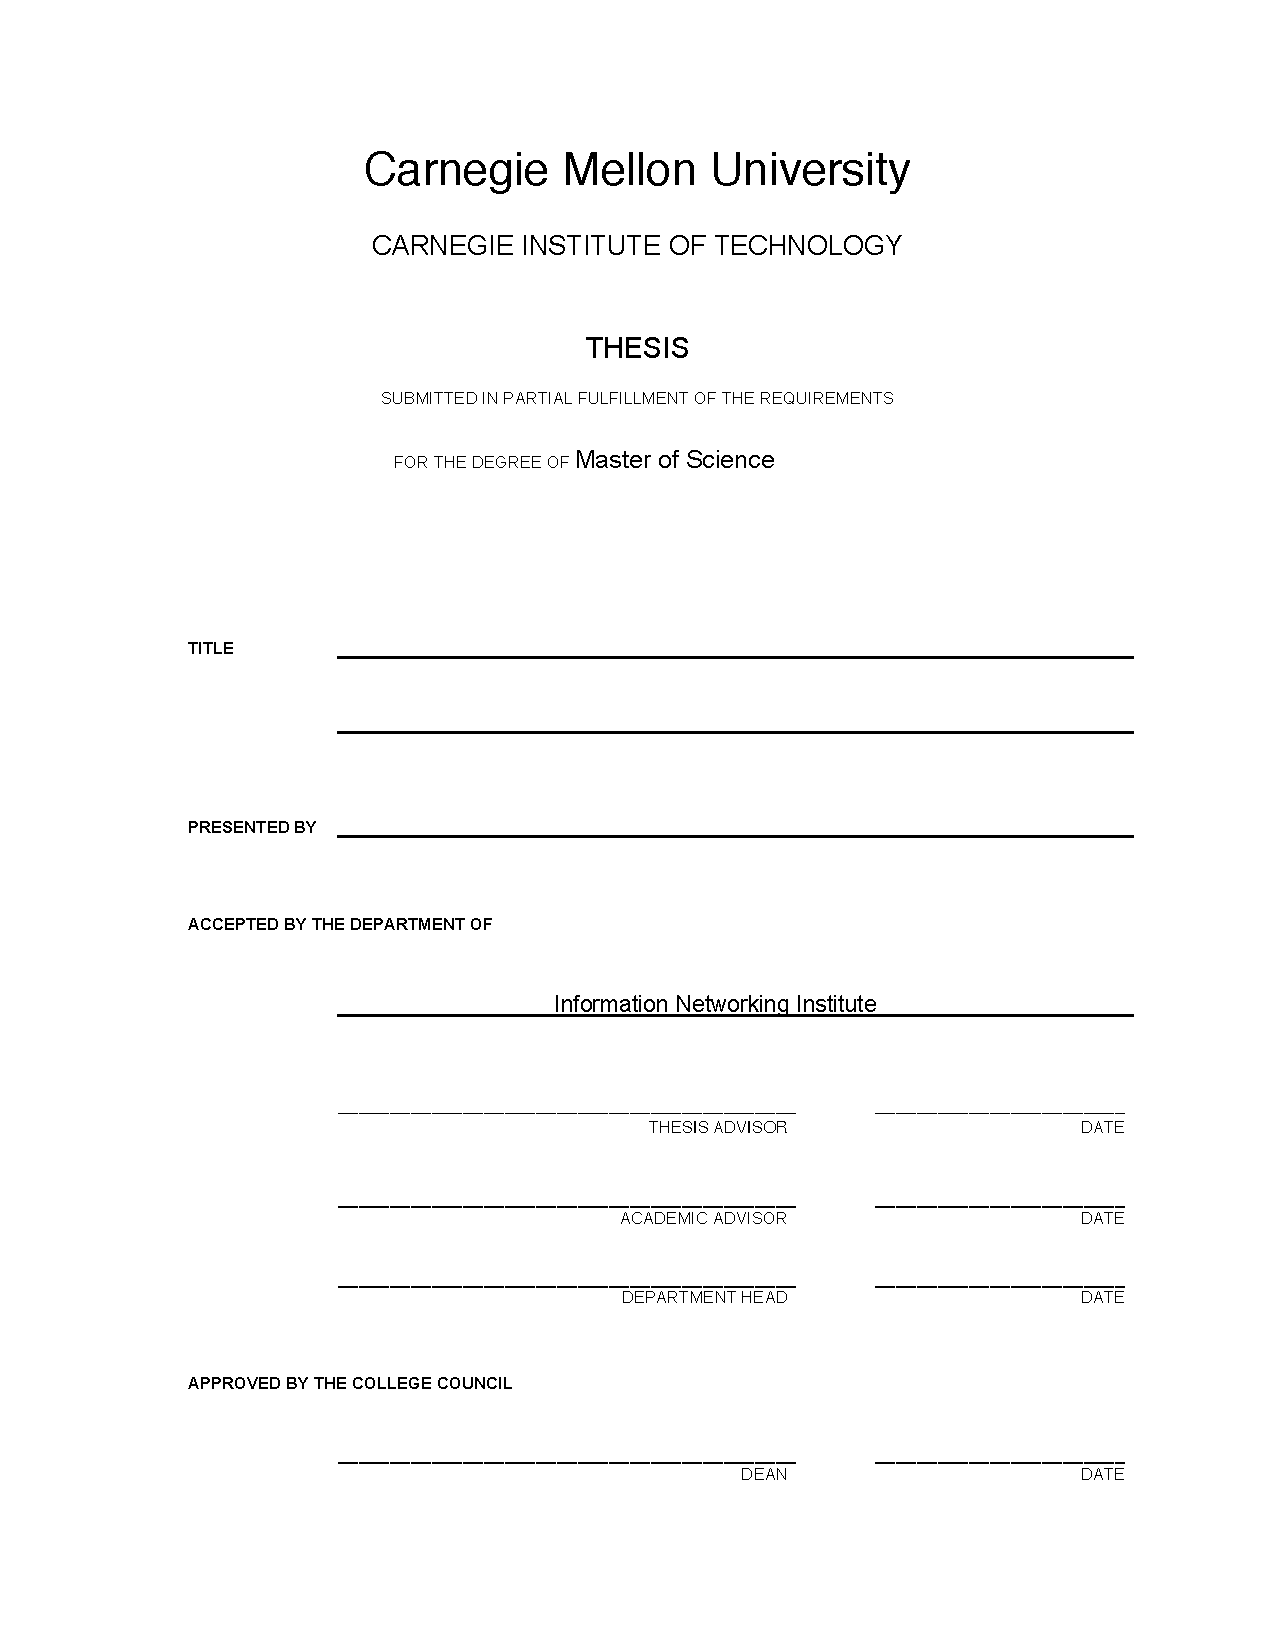
\includepdf[pages={1}]{signature.pdf}

%-----------------------------------------------------------------------------%
% TITLE PAGE -- provides UMI abstract title page & copyright if appropriate
%-----------------------------------------------------------------------------%
\maketitle

%-----------------------------------------------------------------------------%
% ACKNOWLEDGEMENTS -- included file should start with '\acknowledgements'
%-----------------------------------------------------------------------------%
\acknowledgements

\setcounter{page}{2}

Thank anyone you like here.  It's good practice to thank every granting agency that's given you money
since you've been working on your research, any other school you visited during your research,
and any professional society that's funded your travel.
}

%-----------------------------------------------------------------------------%
% ABSTRACT -- included file should start with '\abstract'.
%-----------------------------------------------------------------------------%
\abstract

Write your abstract here.  You should not include references or mathematical notation.}

%-----------------------------------------------------------------------------%
% FRONTMATTER -- ToC is required, LoT and LoF are required if you have any
% tables or figures, respectively. List of Abbreviations and Symbols is 
% optional.
%-----------------------------------------------------------------------------%
\tableofcontents % Automatically generated
\newpage
\listoftables	% If you have any tables, automatically generated
\addcontentsline{toc}{chapter}{List of Tables}%
\newpage
\listoffigures	% If you have any figures, automatically generated
\addcontentsline{toc}{chapter}{List of Figures}%
\newpage
\abbreviations

% You can put here what you like, but here's an example
%Note the use of starred section commands here to produce proper division
%headers without bad '0.1' numbers or entries into the Table of Contents.
%Using the {\verb \begin{symbollist} } environment ensures that entries are
%properly spaced.

\section*{Symbols}

Put general notes about symbol usage in text here.  Notice this text is
double-spaced, as required.

\begin{symbollist}
	\item[$\mathbb{X}$] A blackboard bold $X$.  Neat.
	% Optional item argument makes the symbol/abbr
	\item[$\mathcal{X}$] A caligraphic $X$.  Neat.
	\item[$\mathfrak{X}$] A fraktur $X$.  Neat.
	\item[$\mathbf{X}$] A boldface $X$.
	\item[$\mathsf{X}$] A sans-serif $X$. Bad notation.
	\item[$\mathrm{X}$] A roman $X$.
\end{symbollist}

\section*{Abbreviations}

Long lines in the \texttt{symbollist} environment are single spaced, like in
the other front matter tables.

\begin{symbollist}
	\item[AR] Aqua Regia, also known as hydrocloric acid plus a splash of 
	nitric acid.
	\item[SHORT] Notice the change in alignment caused by the label width
	between this list and the one above.  Also notice that this multiline
	description is properly spaced. 
	\item[OMFGTXTMSG4ME] Abbreviations/Symbols in the item are limited to
	about a quarter of the textwidth, so don't pack too much in there.
	You'll bust the margins and it looks really bad.
\end{symbollist}
} % List of Abbreviations. Start file with '\abbreviations'

%==============================================================================
%-----------------------------------------------------------------------------%
%
% MAIN BODY OF PAPER
%
%
%-----------------------------------------------------------------------------%
\chapter{Introduction}
\label{sec:intro}

Type your introduction here.  This is ``technically'' your first chapter of the dissertation/thesis.}
\chapter{Background}
\label{sec:background}

This chapter is an example of how to format normal material in the
dissertation style.  Most of this information is standard to \LaTeX.

\section{Intra-chapter divisions: Sections}

Section headlines are {\verb"\Large"} and in the standard font. Compare them
to subsections below.

\subsection{Subsections: Wow! Italics!}

Yes, italics.  You may now dance.  Isn't it funny that upright letters are
called ``roman'' while slanted letters are ``italic''.  That's like Italian,
and Romans are Italians too.  What gives?  

\subsubsection{Subsubsections: Smaller and smaller}

Subsubsections are allowed, but are not numbered and don't appear in the
table of contents.  Likewise, you can use the next level of sectioning.

\paragraph{Paragraphs} These divisions are
unnumbered and do not appear in the Table of Contents.
\subparagraph{Subparagraphs} This is the finest division possible.  It's also
unnumbered and omitted from the Table of Contents.


\section{Let's do some math}
Let's look at an equation:
\begin{equation}
\label{eq:diffeq}
\partial{f}{t} = f(t) \quad \text{subject to} \quad f(0) = c.
\end{equation}
We've used the {\verb"\newcommand"} defined in the preamble of 
{\verb"dissertation.tex"} to produce the derivative.  You can get a second
derivative like $\partial{^2 f}{t^2}$ by adding some sneaky superscripts.  Fancy.  

More advanced equation formatting is available in the AMS environments.  See
the guide \href{ftp://ftp.ams.org/pub/tex/doc/amsmath/amsldoc.pdf}{amsmath
user's guide}.  Here are some nice examples of cases people usually have
trouble with.

An equation that's too long for one line --- use \texttt{multline}:
\begin{multline}
	a +b+c+d+e+f+g+h+i+j+k+l+m+n+o\\ 
	= p+q+r+s+t+u+v+w+x+y+z.
\end{multline}
An equation with multiple parts and one number per line --- use
\texttt{align}:
\begin{align}
	a_1 &= b_1 + c_1\\
	a_2 &= b_2 + c_2.
\end{align}
The same equation, set inside the \texttt{subequations} environment:
\begin{subequations}
	\label{hello}
	\begin{align}
		\label{goodbye}
		a_1 &= b_1 + c_1\\
		\label{goodbye_b}
		a_2 &= b_2 + c_2.
	\end{align}
\end{subequations}
Notice that by clever placement of labels, I can reference the pair via
\eqref{hello}, the first \eqref{goodbye}, or the second \eqref{goodbye_b}.
One number for multiple equations can be accomplished using the
\texttt{split} environment:
\begin{equation}
	\begin{split}
		a &= b + c - d\\
		 &\phantom{=} + e - f\\
		 &= g + h\\
		 &= i.
	\end{split}
\end{equation}
People often struggle under the complicated and ugly 'eqnarray' environment.
Don't do it!  The AMS ones are easy.  Other stumbling blocks are cases:
\begin{equation}
	a = \begin{cases}
		b & \text{for $ x > 0$}\\
		c & \text{otherwise,}
	\end{cases}
\end{equation}
matrices:
\begin{equation}
	A = \begin{pmatrix} a_{11} & a_{12} \\ a_{21} & a_{22} \end{pmatrix}
     = \begin{bmatrix} a_{11} & a_{12} \\ a_{21} & a_{22} \end{bmatrix},
\end{equation}
and evaluation bars:
\begin{equation}
	a = \frac{\partial u}{\partial x}\bigg\lvert_{x=0}.
	% Note: if you do this a lot, consider defining a command
	% 'eval' to format this the same every time.
\end{equation}
See the source file for details.

When we reference an equation with something like 
{\verb!\eqref!} 
\eqref{eq:diffeq}. If you
click on the above references in the PDF, your viewer should scroll up to
the above equation. It's handy. 
Labels and references may be attached to all
sorts of objects.  There is a {\verb!\label!} attached to this chapter (it
appears at the top of this file), and we may reference it by
({\verb!Chapter~\ref{chap:example}!}), producing
``Chapter~\ref{chap:example}''.  By default these ref's are hyperlinked as
well.  Later, we'll see labeled and referenced figures and tables.
Particular pages may be labeled with standard {\verb!\label!} commands in
the text and referenced via {\verb!\pageref!}.

You might also like the links from 
{\verb!\cite!} commands to the corresponding bibliographic entry.
Go look at this imaginary book by Stephen Colbert \cite{fancy}.  If you're
not a bibtex expert, look in \texttt{mybib.bib} at the {\verb!@ARTICLE!}
that generated this entry.  It shows an example of accents on author names
and how to preserve upper-case for letters in the title.  Other entries show
the use of the {\verb"and"} keyword between author names.  You may order a
particular author's name as either ``first last'' or as ``last, first''.
The actual format of the bibliography is controlled by the 
{\verb"\bibliographystyle{}"} command in \texttt{dissertation.tex}.


\section{Table of Contents Behavior}
Now is a good time to look back at the Table of Contents.  Notice that you
may click on entries here to warp to the corresponding document location.
In Adobe Acrobat and many other viewers, you can open a 'bookmarks' pane.
This should be populated with named and numbered sections and subsections
identical to the Table of Contents. 

\section{Figures and footnotes}

Figures are set with very little space between the caption and the bottom of
the included graphic.  This is because most graphics programs pad the edges
of images.  If you find the spacing unsatisfactory, you may always add a bit
manually.  The text of the caption is single-spaced, and the word 'Figure'
is set in small caps.  See \ref{fig:example}.  Notice the use of the
nonbreakable space ``{\verb!~!}'' between the ``Fig.'' and the reference.
%%%%%%%%%%%%%%%
\begin{figure}[tbp]
\begin{center}

\includegraphics[width=3in]{inilogo}
\end{center}
\caption[Short caption for table of figures.]{Longer caption for actual body
of dissertation.  Figure captions should be BELOW the figure.}
\label{fig:example}
\end{figure}
%%%%%%%%%%%%%%
Figures (and tables) are examples of 'floats --- objects that \LaTeX decides
where to place for you.  You may give \LaTeX some hints.  Change the 
{\verb"\begin{figure}[tbp]"} to a {\verb"\begin{figure}[b!]"} to restrict the
placement.  Inside the [ ], you can put the following
\begin{itemize}
\item[t] Allow placement at the top of the page
\item[b] Allow placement at the bottom of the page
\item[h] Allow placement 'here', in the middle of the page close to the text
that the figure environment appears next to.
\item[p] Allow placement on a seperate 'floats page' that has no body text.
\item[!] Tighten the screws on the placement algorithm.  This doesn't force
	things to happen as you say, but it makes it much more likely.  
	Be careful: the bang option can cause figures
   to appear above the chapter title and in other bad locations.
\end{itemize}
Notice that each entry just changes what is \emph{allowed}, 
but no preference among
the entries can be registered.  The default is [tbp], which is a very good
default for a document like this, since floats in the middle of a page trap
too much whitespace for double-spaced text. There is also a prohibition against
having a page with more than 75\% float.  Instead, long floats will
get kicked over onto float pages.  Float pages are often a bad idea, as the
creation of one will often cause a domino effect, with all subsequent
figures appearing on float pages themselves, and all these float pages
appearing together at the end of the chapter.  (This is more like sinking
than floating.)  Avoid this by physically moving where the figure environment
appears in your source file to an earlier location.  Don't be afraid to put the environment before
the first spot you reference it!  Many float problems can be solved by a
combination of relocating the figure environment and a little fiddling with the [ ] options.

Also notice the order of the graphic, caption, and label.  If you deviate
from this, strange things can happen.  The caption of this figure shows the
use of short captions (inside []).  These caption appear in the List of
Tables, while the { } captions appear in the body.  If you omit the [ ]
short caption, the long caption will be used in its place.

Another technical note: since this style sheet is designed for processing
by pdflatex, {\verb"\includegraphics"} looks for \texttt{PDF}s,
\texttt{PNG}s, and \texttt{JPG}s instead of the usual \texttt{PS},
\texttt{EPS}, and \texttt{TIFF} formats.  You can convert existing graphics
with a vareity of tools.  \texttt{PDF} graphics are preferred, as they
scale nicely.  The open-source software Inkscape runs on Mac OSX, Windows,
Linux, and some \textsc{UNIX} variants.  Versions 0.46 and beyond have great
support for creating and editing \texttt{PDF}s.  It can even be used to
convert other docs.

\subsection{List of Figures}
If you've put even one measly figure in your document, grad school rules say
you need a List of Figures.  It's automatically generated for you if you do
a {\verb!\listoffigures!} in the master file (heck, it's there right now).
Go look at the list of figures now.  You should be able to click on the
figure number to warp to the figure.  You'll also see the result of the
'short caption' used above.


\section{Table example}

Just to make sure tables are formatted correctly, 
here's an example of a table float, see Table~\ref{tab:example}.
%%%%%%%%%%%
\begin{table}[t]
	\label{tab:example}
	\begin{center}
	\begin{tabular}{c|c|c}
			\hline
			Numbers & Letters & Symbols \\ \hline
			1 & a & $\dagger$ \\
			2 & b & $\ddot \smile$ \\
			3 & c & $\times$ \\
			4 & d & $\sharp$
	\end{tabular}
	\caption{This is an example table}
	\end{center}
\end{table}
%%%%%%%%%%%%%
You should note that [b] formatting 
({\verb!\begin{table}[b]!})
can cause floats to appear under the
footnotes.  Try changing it here and see the ugliness.  Tables are identical
to figures, except that the word 'Table' appears in the caption and its
entry is in the List of Tables instead of the List of Figures.

\subsection{Footnotes}
Footnotes are allowed.\footnote{But, you should probably just work them into
the text since it's annoying to jump around when reading.} They are
numbered with arabic numerals inside each chapter and appear at the bottom
of the page.\footnote{\ldots rather than the end of the chapter or the
thesis.  Those would properly be endnotes, I guess.}  The little footnote
numbers are also hyperlinks.  Try clicking them.  You should place the
footnote command immediately following the period of the sentence it is
attached to.  Any spaces or newlines will result in strange spacing between
the number and the sentence.

\section{Corner cases in formatting, such as very very very long section
titles.  Man, this goes on forever.}

Common corner-cases involve very long titles (like above).  In these cases,
the long titles are set single-spaced both here and in the Table of
Contents.

\subsection{Figure and Table caption cases are neat, and this is an absurdly
long subsection heading}
\label{sec:fig-tab}

Consider the shield logo again with an absurd caption, as in
Fig.~\ref{fig:shield}.
Also examine the new table, Table~\ref{tab:long-caption}.  Both of these
have been forced onto a floats page so you can see what that looks like.
\begin{figure}[p]
	\begin{center}
	
\includegraphics[height=1.5in]{inilogo}
	\end{center}
	\caption{The INI logo again, but now with a really long rambling
	caption.  This caption should be set single-spaced in the LoF and in the
	body text.  What do you think about having graphics in the main directory
	of a project?  I'd prefer them in a folder, then put
	'foldername/picturename' as the argument to includegraphics.}
	\label{fig:shield}
\end{figure}
%%%%%%%%%%%
\begin{table}[p]
	\label{tab:long-caption}
	\begin{center}
		\begin{tabular}{c|c|c}
			\hline
			Numbers & Letters & Symbols \\ \hline
			1 & a & $\dagger$ \\
			2 & b & $\ddot \smile$ \\
			3 & c & $\times$ \\
			4 & d & $\sharp$ \\
	\end{tabular}
	\caption{The same silly table again, but with a really really really
	really really really
	really really really
	really really really
	really really really
	really really really
	really really really
	long caption.}
	\end{center}
\end{table}
%%%%%%%%%%%%%

} % A regular chapter, starts with '\chapter{Title}'
\chapter{Nonsense text for layout proofing}
\label{hello}

Enjoy some Lorem Ipsum text!
This should create about two full pages of text so you can verify the
margins are correct (especially if you're doing two-sided).

\section{Lorem Ipsum}
Lorem ipsum dolor sit amet, consectetuer adipiscing elit. Sed vitae leo.
Pellentesque quis nisi id orci consectetuer posuere. Quisque malesuada
rhoncus dui. Vivamus mi. Mauris commodo. Phasellus lacus magna, feugiat ac,
blandit ut, rutrum id, massa. In consectetuer magna vel justo. Cras eu
diam. Nullam tortor turpis, bibendum non, consequat ac, tincidunt non,
nisi. 

Curabitur sagittis dignissim arcu. Pellentesque habitant morbi
tristique senectus et netus et malesuada fames ac turpis egestas.
Vestibulum ullamcorper. Curabitur faucibus euismod nulla. Vivamus sagittis.
Sed fermentum neque a risus vestibulum convallis. Morbi id massa ut arcu
mollis commodo. Aliquam erat volutpat.  Pellentesque fringilla pellentesque
nisi. Morbi tristique ornare libero. Vestibulum turpis sapien, iaculis ut,
cursus non, condimentum in, tortor. Aenean vehicula. Integer egestas
tincidunt erat. Aenean euismod ante vel lectus. Duis ac sapien vel erat
euismod aliquet. Vivamus tempor placerat nibh. Curabitur pharetra, orci
consequat pulvinar ultricies, orci enim tempor augue, non lacinia orci nisl
et nibh. Nunc gravida dictum turpis.  Duis sollicitudin commodo massa. Nam
ac nunc. Fusce sodales posuere velit. Nunc ullamcorper sodales urna. Donec
consectetuer accumsan ante. Morbi feugiat rutrum mauris. Praesent malesuada
auctor est. Pellentesque quis odio non nulla ornare imperdiet. Aliquam
dapibus. Suspendisse posuere, magna in molestie varius, ipsum velit rhoncus
nisi, nec bibendum pede mauris in urna. Morbi purus lectus, molestie quis,
laoreet id, tincidunt at, ligula. 

Praesent sit amet libero id arcu
adipiscing tristique. Quisque libero erat, bibendum nec, malesuada in,
gravida et, urna. Phasellus molestie vulputate nisi. Nullam massa magna,
dignissim ac, accumsan a, scelerisque eu, erat. Nam tellus augue, tempus
nec, molestie sit amet, rhoncus vel, libero. Vestibulum at neque. Aliquam
laoreet tincidunt mi. Ut laoreet ligula ac urna. Nullam nisl pede, posuere
id, dictum a, fermentum vitae, turpis.  Nulla ante mauris, euismod et,
mollis eu, tempor in, quam. 

In pede augue, elementum varius, tincidunt in,
condimentum ut, erat. Etiam vulputate faucibus velit. Aliquam porttitor.
Nam fringilla adipiscing nisi. Sed in magna. Aenean non ante. Aenean
facilisis, nunc sed aliquam porta, magna est aliquam nisi, vitae semper
turpis orci ac dolor. Praesent nec tellus. Cras vulputate rhoncus sem.
Curabitur eu mi. Mauris euismod lacinia nibh. Suspendisse eget sapien et
nunc accumsan elementum.  Nulla dapibus. Donec interdum elit mattis velit
imperdiet aliquet. Mauris feugiat, ante vel faucibus rutrum, eros mauris
sollicitudin neque, ut varius diam ipsum et massa. Nullam non nisi sit amet
tortor rhoncus molestie. Cras consectetuer condimentum ante. Phasellus
fermentum risus fermentum turpis. Mauris dignissim iaculis sem. Fusce nisi
lorem, viverra id, auctor et, scelerisque ut, massa. In hac habitasse
platea dictumst. Vestibulum ante ipsum primis in faucibus orci luctus et
ultrices posuere cubilia Curae; Aliquam pulvinar neque ac dolor.

\section{More nonsense}
Lorem ipsum dolor sit amet, consectetuer adipiscing elit. Sed vitae leo.
Pellentesque quis nisi id orci consectetuer posuere. Quisque malesuada
rhoncus dui. Vivamus mi. Mauris commodo. Phasellus lacus magna, feugiat ac,
blandit ut, rutrum id, massa. In consectetuer magna vel justo. Cras eu
diam. Nullam tortor turpis, bibendum non, consequat ac, tincidunt non,
nisi. 
Curabitur sagittis dignissim arcu. Pellentesque habitant morbi
tristique senectus et netus et malesuada fames ac turpis egestas.

Vestibulum ullamcorper. Curabitur faucibus euismod nulla. Vivamus sagittis.
Sed fermentum neque a risus vestibulum convallis. Morbi id massa ut arcu
mollis commodo. Aliquam erat volutpat.  Pellentesque fringilla pellentesque
nisi. Morbi tristique ornare libero. Vestibulum turpis sapien, iaculis ut,
cursus non, condimentum in, tortor. Aenean vehicula. 

Integer egestas
tincidunt erat. Aenean euismod ante vel lectus. Duis ac sapien vel erat
euismod aliquet. Vivamus tempor placerat nibh. Curabitur pharetra, orci
consequat pulvinar ultricies, orci enim tempor augue, non lacinia orci nisl
et nibh. Nunc gravida dictum turpis.  Duis sollicitudin commodo massa. Nam
ac nunc. Fusce sodales posuere velit. Nunc ullamcorper sodales urna. Donec
consectetuer accumsan ante. Morbi feugiat rutrum mauris. Praesent malesuada
auctor est. 

Pellentesque quis odio non nulla ornare imperdiet. Aliquam
dapibus. Suspendisse posuere, magna in molestie varius, ipsum velit rhoncus
nisi, nec bibendum pede mauris in urna. Morbi purus lectus, molestie quis,
laoreet id, tincidunt at, ligula. 
Praesent sit amet libero id arcu
adipiscing tristique. Quisque libero erat, bibendum nec, malesuada in,
gravida et, urna. Phasellus molestie vulputate nisi. Nullam massa magna,
dignissim ac, accumsan a, scelerisque eu, erat. Nam tellus augue, tempus
nec, molestie sit amet, rhoncus vel, libero. Vestibulum at neque. Aliquam
laoreet tincidunt mi. Ut laoreet ligula ac urna. Nullam nisl pede, posuere
id, dictum a, fermentum vitae, turpis.  Nulla ante mauris, euismod et,
mollis eu, tempor in, quam. 
In pede augue, elementum varius, tincidunt in,
condimentum ut, erat. Etiam vulputate faucibus velit. Aliquam porttitor.

Nam fringilla adipiscing nisi. Sed in magna. Aenean non ante. Aenean
facilisis, nunc sed aliquam porta, magna est aliquam nisi, vitae semper
turpis orci ac dolor. Praesent nec tellus. Cras vulputate rhoncus sem.
Curabitur eu mi. Mauris euismod lacinia nibh. Suspendisse eget sapien et
nunc accumsan elementum.  Nulla dapibus. Donec interdum elit mattis velit
imperdiet aliquet. Mauris feugiat, ante vel faucibus rutrum, eros mauris
sollicitudin neque, ut varius diam ipsum et massa. Nullam non nisi sit amet
tortor rhoncus molestie. Cras consectetuer condimentum ante. Phasellus
fermentum risus fermentum turpis. Mauris dignissim iaculis sem. Fusce nisi
lorem, viverra id, auctor et, scelerisque ut, massa. In hac habitasse
platea dictumst. Vestibulum ante ipsum primis in faucibus orci luctus et
ultrices posuere cubilia Curae; Aliquam pulvinar neque ac dolor.
}
\chapter{Overview}
\label{sec:overview}

Ea dico populo saperet nam, atqui mundi viris et vim. Te choro aperiri vim.

Duo ignota nonummy ei. Ex augue latine luptatum eum. Omnesque scaevola vis
ne, erat perpetua convenire ius in. Duo cu movet sonet corrumpit. Ex eos
reque prodesset.\ref{hello}

In sint veritus singulis pro, at audire regione luptatum eam. Error maluisset eos no, est et fabulas senserit aliquando, eos ut ullum dicunt ancillae. Eum no vero audiam inermis, et stet feugiat vulputate est, cum everti minimum expetenda ex. Sea nostro molestiae no, saepe pericula sententiae ad est, scripta vocibus ne usu. Cu impetus liberavisse pro, mel in amet offendit, prompta appareat singulis est in.

Te labitur petentium quaerendum sed, ut pro ipsum saepe splendide. Vel cu quidam facilisis, usu harum possit alienum ad. His id fuisset pertinax, ea diceret periculis principes mel. Cu vis aeque utamur deleniti, simul salutatus voluptaria vim cu. Stet natum decore ut eum, mel nulla tibique et. Et sit commodo conceptam accommodare, per at altera impedit albucius.

\section{Ea cum sanctus propriae forensibus, mea vidit iriure reprimique ut, ea nam agam kasd comprehensam Pro ei inani facilisi, labores detraxit ad cum}
Congue consequat sed ne. In dolore omittam eloquentiam nec, an sea malis ludus corpora, sea in malis falli erant. Id veniam persequeris eam. Augue inani nemore usu at, sea an reque dicam, vis porro animal in. Alii dolorem prodesset quo eu.

Eu aeque definiebas voluptatibus pri. Vel ne meliore elaboraret, propriae scaevola omittantur an mei. His ei mucius ornatus delicata, diam etiam patrioque ea sed. Ut eos persius intellegam dissentiunt, causae impedit te mei. Torquatos signiferumque ut quo.

Vix nibh volutpat ad, an cum mutat facer possit. Pro possit causae facilis ex. Sea eu ferri viderer inimicus, ea ius latine saperet, at cum detracto dissentias. Mea ex epicurei atomorum mandamus, an his dicam molestiae. Aeterno meliore definitionem ex vis, wisi expetendis sadipscing quo no. Eos inermis accumsan ne.

Modo tritani ea duo, vis mazim affert argumentum no. Usu ne ferri utamur nominati. Mei ad modo oportere. Brute minim scribentur ex cum, te vel agam epicuri consetetur. Ea vel mundi ridens inimicus, ad eruditi interpretaris mea, eum eu ferri rebum lorem. Dolore populo quaeque sit ex.

In accusata urbanitas vituperata quo, consulatu torquatos eam ex, tota definitionem quo et. Atqui suscipit suavitate at sea, intellegam theophrastus qui no, te homero temporibus per. Id meis mucius petentium usu, cu nam sonet elaboraret. Sumo accommodare cu pro, ne ornatus delectus consulatu duo, exerci laboramus assentior duo et.

Ea eos dicat everti appetere. Tota lorem scribentur ius ad, an possim noluisse adversarium pro. Everti adipiscing voluptatibus ius an, in ullamcorper necessitatibus vis. Te pro nibh invenire, porro putant salutandi quo ad. Id exerci equidem suavitate nec, cu sed erat veniam postea. In tale facilisi posidonium per, pri suscipit deterruisset an.


\section{Ipsum}
Lorem ipsum vis at liber dicit diceret. Id fierent omittam est, vis natum electram eu, prompta sensibus at vix. Ut mea modus novum reprimique, vel euismod referrentur an. Ne legimus placerat abhorreant nec, no deleniti interesset vis. Vel adhuc graeci cu, ea est graecis fabellas.

Vel ex facer suscipiantur definitiones, mea vituperatoribus sale porro no, ut aliquip disputando sit. Ad graece albucius oporteat nec, vim voluptatum interesset in. Autem mundi eos ei, omnesque voluptaria et pri, falli quaerendum quo cu. Dicit equidem ceteros ne duo, ad oratio nostrud fierent usu, ei aliquyam periculis intellegam vim. Audiam principes sententiae sed et, ex his dicant facilis. Posse primis melius an per, quod assueverit duo id, cu usu animal propriae.

An natum nemore est, et eum quidam semper voluptua, meliore euripidis ei sea. Mei mutat invidunt ex. Vix choro delicata te. Causae mediocrem an his, choro vidisse id est. Mundi dolor id mei, an duo tation omittam.

Ex magna facer torquatos vel. Te pro sumo legere consequat, duo ea luptatum phaedrum. Nec in laboramus interesset cotidieque, deleniti vivendum ex eam, at senserit hendrerit vel. Est rebum falli ad, cu latine viderer efficiendi nec. Vidisse delectus te mei. Eu sanctus patrioque philosophia usu.

At veniam malorum iuvaret his, eos soluta ullamcorper ut. Zzril integre sit ut, sed regione percipitur contentiones et, mea no aliquyam efficiendi. Vix et neglegentur definitiones, ne graeco dictas omittam est. Id mel eros soluta corrumpit, oportere torquatos vim an.

An est eligendi efficiendi intellegam, illud putent labitur eu duo. Id fabellas salutatus argumentum has. Qui malorum prompta ex, eu sea nostrud admodum sensibus. Ex tamquam complectitur has, diceret volumus eam cu. Eam nusquam deleniti ponderum cu. No eam tale moderatius.

Est saepe dicam abhorreant ut, omnes soleat quo no. Duo ceteros pericula interesset ut. Nec eu iudico option, persius euismod no eum. Per ea luptatum oporteat qualisque.

Dico veri nec ei, est ne audiam graecis corrumpit. Dico possit an pri, illum feugiat cum ne, ne duo lorem corpora platonem. Cum no aeque feugait, in vis odio nihil. Iusto sadipscing scriptorem ne est. Ius ad salutandi intellegebat.

Nonummy mentitum his an, viris maiorum assentior pri cu, duo errem partiendo quaerendum ad. Cum aperiam sententiae ex. Dolor salutandi pro in, nec ei utinam causae, praesent concludaturque quo te. Id fuisset consequat eum, vide eirmod qui et. Cu tollit ubique concludaturque has, his id sale consectetuer, eu mel discere scripserit. Mei diceret efficiantur eu, no sea doctus meliore reformidans.

Nihil accommodare sit ea, nec et mutat dolorum. Ut conceptam persequeris vis, ea luptatum consetetur nam. Vix ea deleniti evertitur. Has enim consequat id, falli clita duo an.
}
%%
% $Id: methodology.tex 164 2010-12-08 21:26:36Z nicolasc $
%

\chapter{Individual Analysis}
\label{sec:implementation}
%
%-	All the devices could boot into recovery mode, so we used the recovery technique \cite{Tim}
%-	Android boot image structure
%	¥	Header Ð defines the size of each segment of the boot image, where to flash each segment in memory, and gives command line options to the bootloader
%	¥	Kernel Ð the kernel that is run by the bootloader when the device boots into recovery mode
%	¥	Ramdisk Ð basically a small filesystem that contains the files necessary to start the system.
%- 	Built a custom image for each device, reduced, and compared
%	¥	Used source.android.com to build the ramdisk
%	¥	Used source from manufacturers, stock images, or mod images to get kernel and header

To generalize the recovery method for Android, we focus on two key components:  the recovery image and the flashing mechanism.  In this section we will further discuss the components of the recovery method and give the steps taken to port the recovery method to each device.

\section{Recovery Image Structure}
\label{sec:boot_image}	


The first step in porting the recovery method to a new device is better understanding the recovery image.  The recovery image consists of three main components: the header, kernel, and the ramdisk \footnote{A secondary ramdisk is optional, however it is unnecessary to our application and for simplicity has been omitted from our discussion}.  The Android bootimg structure can be seen in Figure \ref{fig:bootimg_struct}. 

\begin{figure*}[!t]
\centering
\includegraphics[width=0.8\textwidth]{Pictures/bootimg_struct}
%\includegraphics[width=3in]{figs/motomotog1}
\caption{\label{fig:bootimg_struct}
{\bf Bootimg Structure}: structure of a common Android bootimg}
\end{figure*}

\begin{figure*}[!t]
\centering
\includegraphics[width=0.7\textwidth]{Pictures/header_struct}
%\includegraphics[width=3in]{figs/motomotog1}
\caption{\label{fig:header_struct}
{\bf Header Structure}: structure of a common Android bootimg header}
\end{figure*}
	 
\subsection{Header}
\label{sec:header}

The first segment of an Android recovery image is the header.  The header is placed at the start of the image and provides essential metadata to the bootloader for loading the other components when booting into recovery mode.  The structure of the header is given in bootimg.h\footnote{bootimg.h can be found at $<$path to source tree$>$/system/core/mkbootimg/bootimg.h} in the Android source \cite{_welcome_????} and can be seen in Figure \ref{fig:header_struct}.

The image header begins with the magic signature ("ANDROID!"), which is used to identify the start of the image.  After the magic signature, the size and memory location in which to load the kernel, ramdisk, and secondary image is given.  The header concludes with the physical address of any kernel tags, the image's page size, command line options, and a checksum which is used to detect whether the recovery image has been corrupted.

\subsection{Kernel}
\label{sec:kernel}

The second segment of the recovery image is a gzipped kernel.  As described in Section \ref{sec:ekernel}, the kernel stored in the recovery image is a customized variant of the Linux 2.6 kernel.  The kernel acts as a mediary between the Android framework and the hardware, memory management, process management, the network stack, and the driver model \cite{android_developers}, so the kernel for each device is tuned to work with a specific set of hardware.

\subsection{Ramdisk}
\label{sec:ramdisk}

\begin{table*}[!t]
\begin{center}
\small
\begin{tabular}{|c|c|}
\hline
 {\bf Name}  & {\bf Description} \\
\hline
\hline
default.prop & Default Build Properties \\
\hline
init.rc & System-wide initialization values  \\
\hline
init & Initialization executable  \\
\hline
system/ & System files and tools   \\
\hline
sbin/ & Additional tools   \\
\hline
sbin/adb & Android Debug Bridge executable   \\
\hline
sbin/recovery & Recovery executalbe  \\
\hline
res/ & Images for recovery mode \\
\hline
\end{tabular}
\end{center}
\caption{Important Ramdisk Files}
\label{table:ramdisk_files}
\end{table*}

The last segment of the recovery image is the ramdisk.  The ramdisk in the bootimg is a compressed (gzip or lmza) cpio file containing an initial directory structure for the kernel \cite{android_developers}.  Essentially, the ramdisk contains the core files needed for system initialization.   Table \ref{table:ramdisk_files} gives the files and folders most commonly found and important in the recovery image and their usage.  The most important files are the \emph{init} binary, \emph{init.rc}, which controls most system-wide properties, and the \emph{recovery} binary, which is executed when the phone is booted into recovery mode \cite{rootzwiki_unpack}.

Note that though the image structure given above is defined by the Android framework, not every device uses the same image structure.  Specifically, Samsung devices use a different method where the ramdisk is built into the kernel and the kernel is then flashed on to the device.  However, the components for each method remain the same, the only difference is in the way they are packaged.

\section{Custom Image}
\label{sec:custom_image}

To build a custom recovery image for each device, we split the process between the three components of the image: the header, kernel, and ramdisk.

\subsection{Header}
\label{sec:custom_header}

To generate a header for our new recovery image, we need to select values for the size and loading location of the kernel, ramdisk, and secondary ramdisk, the address of the kernel tags, image page size, command line options, and checksum.  We omit the magic signature in our discussion because it is constant across all images.

The sizes for the kernel, ramdisk, and secondary ramdisk can be calculated once we create our custom components as described below\footnote{the size of the secondary ramdisk will always be zero because it is never used in our application}.  The loading location for each component is generated as a standard offset from a base address\footnote{kernel address = base + 0x0000800, ramdisk address = base + 0x01000000, secondary ramdsik address = 0x00F00000, kernel tags address = base + 0x00000100} (given in mkbootimg.c\footnote{mkbootimg.c can be found at $<$path to source tree$>$/system/core/mkbootimg/mkbootimg.c}).  Therefore, we only need to select a single base offset.  Additionally, the checksum is calculated over all our custom components.

To select the correct values for the base address, page size, and command-line options, we can either extract them from another working image's header or from a kernel built for our device.

\subsection{Kernel}
\label{sec:custom_kernel}

For our custom recovery image to work on a new device, we need a kernel that understands how to communicate with the specific hardware found on that device.  Obtaining a working kernel can be done in one of two ways, building the kernel from source or extracting it from a working image.

\subsubsection{Kernel Source}
\label{sec:kernel_source}

Some manufacturers (HTC, Samsung, etc.)\cite{htc_source, samsung_source} have made the kernel source for all their devices publically available.  For these devices, we can simply download their source and an ARM cross-compiler \cite{cross_compiler} and build to get a working kernel.  Note, this method is preferable to extracting a kernel binary because the source can be read and analyzed to ensure that no malicious or unwanted actions are executed when running a kernel, whereas identifying unwanted effects  becomes much more difficult when looking at a kernel binary \cite{enck_app_security}.  

For future analysis and comparison purposes, when building each device kernel we minimize the configuration so that only necessary components are included.  Because our forensic application only requires a small set of features, we removed any unnecessary devices, such as audio, open GL, and networking drivers, and only included code necessary to run the recovery executable, access memory, and establish an \emph{adb} connection over USB.

\subsubsection{Extracted Kernel}
\label{sec:extracted_kernel}

For devices where no source is available, we extracted our kernels from recovery images that are known to work for our target device.  Working images can be obtained through one of three methods.

The first two methods obtain a "stock" image, the image that is provided by the manufacturers for that device.  The first method is to obtain another device that is the same model and is unrelated to the investigation.  With the secondary device, a recovery image can be extracted using a technique similar to those given in Section \ref{sec:rooting}.  The practitioner would root the device, then use a tool like Nandroid Backup \cite{nandroid} to extract the recovery image.

The second method for obtaining a "stock" image is to obtain an Over-the-Air (OTA) update for the device.  To push software updates to devices, Android provides a mechanism for supplying updates wirelessly \cite{android_ota}.  By intercepting OTAs as they are transferred to the device, or querying the Android OTA servers using the proper protocol, it is possible to obtain a stock image, though querying OTA servers may be difficult as it would require impersonating the device \cite{tim_usenix_2012}.  

The final method for obtaining a working recovery image is through the modding community.  "Modded" images, as discussed in Section \ref{sec:mod_comm}, provide a modified Android experience for users that want to push the performance of their devices or add features not supported by Android.  "Modded" images can be obtained from many sources, such as forums \cite{droid_mod_forum, xda_developer_mod_forum, android_modz} and developer sites \cite{cyanogen_wiki, amon_ra_wiki}.  Because of the strong Android development community, images for all devices can typically be found and if a "modded" image is not available, there is commonly a stock image posted by someone attempting to create a "mod" for their device.  Therefore, the modding community can also be useful in finding stock images for devices that can not be procured.  However, posted stock images should not be relied upon unless absolutely necessary as it is hard to know whether the extraction of the image was executed properly and no modifications have been made.

A stock image is preferable to an image from the modding community because Android and the manufacturer are assumed to test the images more thoroughly and are motivated by sales to ensure their code works with no negative effects, whereas "modders" may have other motivations which could lead to unwanted side effects.

\subsection{Ramdisk}
\label{sec:custom_ramdisk}

To generate a custom ramdisk for our recovery image we utilize the openness of the Android platform.  Using the Android source \cite{_welcome_????} we simply modify a few configuration files to match the configuration of our device, and add our forensics tools into the build tree for inclusion into the image.

\subsubsection{Device Configuration}
\label{sec:device_config}

To build a ramdisk for a new device we have to add a folder under the \emph{device/} directory for the manufacturer\footnote{If a device for by the same manufacturer has already been added to the tree, then just use the folder for that manufacturer.} and within the manufacturer directory add a new folder for the device.  The device specific directory contains all the information necessary to build the Android source for a given device.  Configuration information includes all the specific header information given in Section \ref{sec:custom_header}, the custom kernel from Section \ref{sec:custom_kernel}, and other make information necessary for the build process.

To build the ramdisk once configuration information has been given, use the following set of commands:
\begin{quotation}
. build/envsetup.sh

lunch full\_$<$device name$>$-eng

make -j1 recoveryimage
\end{quotation}

The resulting ramdisk can be found at \emph{out/target/product/$<$device name$>$/recove-}\emph{ry/root/} in the Android build directory.  Note, to prepare for device build comparison and analysis we reduce the device configuration to its minimal set of necessary options, to avoid including any spurious information in our analysis.

\subsubsection{Forensic Tools}
\label{sec:forensic_tools}

To add our forensic tools to the ramdisk, we have to make two modifications: add custom busybox source to the build tree and update init.rc.

Busybox is an executable which contains size optimized versions of common Linux tools designed for resource limited systems \cite{busybox_about}.  By adding busybox to the build we provide the \emph{adb} remote shell with commonly used tools such as \emph{ls}, \emph{cat}, \emph{file}, etc with little effort.  Also, busybox is open source and extendable \cite{add_to_busybox}, allowing us to add our forensic tools, such as \emph{nanddump} and \emph{transfer}, into the ramdisk with little effort

To add busybox to the Android build we first copied the modified busybox source into the \emph{external/} directory of the Android source tree.  To get the recovery executable to properly reference busybox we also have to modify recovery.c\footnote{recovery.c can be found at \emph{bootable/recovery/recovery.c} in the Android source tree} to redirect any input to the recovery tool that is not recognized by recovery to busybox and update the make files to include links to busybox and the busybox libraries.

The init.rc file is used to control system-wide properties, such as partition mounting and starting service \cite{rootzwiki_unpack}.  For our forensic application, we modify the init.rc file to mount the partitions we want to image as globally readable, give our forensic tools root level permissions, and ensure that the adb service is running at startup. Our modifications were made to the init.rc file found in \emph{bootable/recovery/etc} in the Android source tree.

\section{Flashing Tools}
\label{sec:flash_tools}

Once we have created an image for each device, we then need to find a way to write the custom image to the recovery partition.  For maintenance purposes, manufacturers tend to build proprietary tools for flashing images, though they may not be publicly available and may require a carrier or manufacture key to use.

\subsection{Acquiring the Tool}
\label{sec:acquiring_tool}

To first obtain the flashing tool there are several possibilities.  If the tool is provided publicly (such as \emph{fastboot} \cite{fastboot}), then it can simply be downloaded from the developer's website and used to write the recovery image.  However, these tools are typically not open source and commonly are only built for the manufacture's operating system of choice (i.e. Windows).  Thus, if the practitioner is using a different operating system, they either need to run the tool in a virtual machine (VM), which can have problems negotiating a connection over USB, or use a different tool.

Many of the proprietary tools have been reverse engineered \cite{sbf_flash, heimdall} by the modding community and distributed publicly for multiple host operating systems.  Modded tools are easier to obtain and avoid the challenges presented by proprietary tools, however, they should still be used with caution, similarly to the images discussed in Section \ref{sec:extracted_kernel}, as they are provided by a less reputable source.  In the case of reverse engineered tools, it is best to find open source implementations, so the source can be analyzed for any negative side effects before use.

\subsection{Locked Bootloader}
\label{sec:locked_bootloader}

After we have the flashing tool it is important to understand what level of privilege we have to write to the device.  In some cases our access may be completely unrestricted.  If we are given full write capabilities, then we can simply connect our device via USB and begin writing our recovery image.  However, this is not always the case.  Some phones may have an unlock-able or signed bootloader which restricts write access to the device.

In the case of an unlock-able bootloader, the manufacturer allows the user to overwrite the device images, but only after they receive a key from the manufacturer.  By requiring a manufacturer key to unlock a device, the manufacturer can identify which devices have been unlocked and thus have voided their warranty. 

The other case of bootloader restriction is the signed bootloader.  With a signed bootloader, only images which are signed by the manufacturer's cryptographic secret key can be written to the device.  By using a signed bootloader, the manufacturer prohibits any updates to the phone's image that they did not create.

For our analysis we bypass bootloader restrictions for the sake of building recovery images for a greater range of devices.  We bypass the unlock-able bootloader simply by registering the devices with the manufacturer to obtain a key and continuing with the unlock process and we circumvent the signed bootloader by exploiting a vulnerability in the operating system.  Specific cases of our techniques will be given in Section \ref{sec:results}.  We assume that in a real forensic investigation, the authority prosecuting the case could obtain the manufacturer key through the legal process to reach the same resultant unlocked state we have achieved without any modifications to the system.
} //Some other possible sections
%\include{{./Chapter6/testing}}
%\include{{./Chapter7/results}}
%\include{{./Chapter8/conclusion}}
%\include{{./Chapter9/discussion}}
%\include{{./Chapter10/future}}
%==============================================================================

%-----------------------------------------------------------------------------%
% BIBLIOGRAPHY -- uncomment \nocite{*} to include items in 'mybib.bib' file
% that aren't cited in the text.  Change the style to match your
% discipline's standards.  Of course, if your bibliography file isn't called
% 'mybib.bib' you might want to change that here too :)
%-----------------------------------------------------------------------------%
%\nocite{*} - if you use this it will put EVERYTHING in your .bib file into the references even if you don't cite it in the text
% \bibliographystyle{./Bibliography/jasa} %Formats bibliography
\bibliographystyle{./Bibliography/IEEEtranS} %Formats bibliography
\cleardoublepage
\normalbaselines %Fixes spacing of bibliography
% \addcontentsline{toc}{chapter}{Bibliography} %adds Bibliography to your table of contents
\bibliography{./Bibliography/References} %your bibliography file - change the path if needed

%-----------------------------------------------------------------------------%
% APPENDICES -- OPTIONAL. These are just chapters enumerated by Appendix 1,
%                Appendix 2, Appendix 3...
%-----------------------------------------------------------------------------%
% \appendix
% \chapter{Populo Ornatus}

Ut quando convenire scripserit mei, ut accusam noluisse eam. At scripta democritum quo, reque everti an qui, posidonium efficiendi ut mel. Pro an reque habemus, augue nemore conceptam in vim. Eu cibo ancillae takimata usu.

No vis albucius rationibus, eum doming ceteros constituto id. Ad suas zzril laudem cum. Natum mollis singulis vel te, ea elit imperdiet duo, odio inermis et eos. Nam ad vocibus tractatos, sit no vidisse diceret omnesque, mollis omnesque ea mea.

Ut est ridens principes scribentur, menandri interesset adversarium ius ut. Ut duo elit dissentias, at sea eleifend scripserit, eam nibh rebum definitiones an. Cum te quaeque epicuri mentitum, his elitr essent et, in sea habeo aliquid convenire. Quo euismod sadipscing definitionem an, ut duo iusto aliquando, graece appetere ne nec.

Consul imperdiet dignissim vis et, mei liber vidisse principes et, eu nam docendi voluptua democritum. Qui no dicat tamquam sanctus, saepe tincidunt no mel. Pro ignota albucius consetetur in, sint qualisque assueverit eam ut, vis graeco denique signiferumque ne. Sale appellantur contentiones eu his, pro magna ornatus ut, ad vidit omnesque euripidis pri. Sea congue moderatius in, his dicit suscipit no, mei ei incorrupte assueverit. Nusquam nominavi et quo, idque delenit vim an, posse quaeque an mea.

Suas elitr lucilius sit an, aeterno persius vel eu. Mel at essent aperiam repudiare. Tale consul eum ne, eam no meis delenit iudicabit, an sint mutat pri. Nec no clita propriae pericula, duo explicari gubergren ei. Ne sit autem nominavi, te falli deserunt per. Quo tractatos suscipiantur ex, electram dignissim usu no, cu congue iriure vivendo vim.

At vero graeci fuisset his, quo similique persequeris ad. Ex est graece mandamus, antiopam voluptatum his ea. Assum appellantur mel an, ei mea veri commune efficiendi. Pri blandit urbanitas no. Nam ex enim reque, ut nec iusto regione ullamcorper, facer harum pertinacia mei ei. Erant veniam imperdiet an eam, veniam mucius equidem ius eu, at scripta labitur est.

Et quo soluta graecis accommodare. Tamquam mentitum menandri vim ut. Ut nec melius senserit, ut mei sale aeque. Prompta delectus mea te, fierent adipisci ad per, mei odio pertinax senserit et. Per ut persius singulis. Id qui malorum iracundia, semper conceptam cu sed.

Vis nominavi urbanitas intellegat an, ut numquam deseruisse sea. Et quo dico aeque adipiscing, ius ea commodo epicurei, eum cu nulla imperdiet efficiantur. Ea cum simul scripserit. Ius reque decore voluptaria ei, nec sensibus mediocrem eu, sit iriure vivendo ad. At munere maiestatis mel, ex persius honestatis nec. Nihil omnes definiebas duo cu, dicat ancillae no vix. No est prompta apeirian, mel ad quaestio theophrastus mediocritatem.

Persequeris intellegebat disputationi et nec, nam ne alia solum reque, ad pri clita appellantur reprehendunt. Clita iracundia ex cum, placerat invidunt dissentias ius id. Possit dictas recteque sed ne. At eam singulis recusabo intellegat, ius in probo clita posidonium, id atqui paulo rationibus pro. Ut elit mucius qui. Mel ea ubique nostrud takimata. Cu eos vituperatoribus temporibus feugait.

Per putent nusquam oportere cu, nullam discere te sea, an vix quot mutat. Cibo reque nostrum nec eu, justo mucius aeterno vis id. Facer tempor cu vix, ex saepe similique maiestatis qui, ne pro eripuit offendit. Id mel cetero efficiantur. Cum homero aeterno euismod an, vulputate definitiones ne quo.

Sed exerci incorrupte et, usu mundi molestiae reformidans in, at probo vocibus quo. Ex vel aliquip maluisset. Qui enim error an, molestie incorrupte an ius. Id maiestatis temporibus mei, tantas oporteat ocurreret id pri. Ei nam velit doming utroque.

Suas vituperata mel eu, ex veri omnes duo, an modo molestie ius. At vis moderatius dissentias scripserit, nullam aliquam usu no. Cibo diceret sed an. Sea cu ridens convenire.

Pro prima blandit no. His ut dicit iriure oblique, eos meis urbanitas abhorreant te. Usu cu perpetua principes. Mutat utinam insolens id cum. Quo tale iudicabit conclusionemque ex. Eos id harum accommodare.

Vel legere liberavisse ut, et aeque timeam usu. Vis eu dico sanctus appetere, id vix graecis repudiare, ad persecuti mnesarchum mei. No atqui nemore deseruisse eum. Meliore accumsan accommodare in qui, an tation rationibus has, ea nulla aliquip euismod his.

Utinam ridens cum eu. Duo aliquam omnesque cu, sea elitr appetere ea. Mea no quas discere apeirian, munere hendrerit conceptam duo an, nec ad habeo tritani. Vis exerci volumus no. Omittantur reprehendunt no has. Malis accusata necessitatibus no nam.

No solet assentior ius, an ferri dissentiet pro, vix ad tantas offendit. Pro tollit consequat gloriatur ne, eu vix amet posidonium. Errem utamur veritus vix ea. Sed laboramus omittantur id, ut sonet voluptatum has, cu doctus iriure menandri eos.

Regione iudicabit ei per. Cum ea aliquip voluptatibus. Sit in partem explicari. Ne probo labores placerat mei. Ullum pertinax ea his, per cu persius impedit adipisci. Fabulas ancillae dignissim ei his, ius no nulla melius suscipiantur, ne vel laudem eripuit gubergren.

Ei qui equidem adolescens. Has ad accusata urbanitas voluptatum, no pri ferri dicit. Ne qui veritus omittam neglegentur, usu et lorem audiam mediocrem. Vim falli dictas labitur cu, dolores laboramus constituto id has, sit ea sint summo utroque.

Mei graecis definiebas eu, ad his brute omittam elaboraret. Ridens laoreet eos ne, diam mnesarchum ne sea. Idque everti ea pro, eruditi probatus patrioque eu has. Cum omnes gubergren ex, cum te noster offendit indoctum. Putant dissentiunt duo ex, dicat etiam cu quo. Duo esse probatus complectitur ex, vitae eripuit nostrum no sed, cum odio veri reformidans ex.

Vide ipsum ei vel, at diam nominavi his. Etiam assueverit nam eu, ut habeo nusquam eleifend mei. Pro eirmod perpetua id, minim urbanitas usu no. Vim elitr nominati definitionem ex. Ex tollit quaerendum has, nonumy inciderint eos ne. Vis posse munere honestatis ut.

Eu ornatus meliore usu, enim aeque possim eu cum. Pri ad everti fabellas, at pro omnium convenire repudiare, ut mel hinc minimum. Eam et puto reque mollis. Sed ad ponderum lobortis, cu pro viris vitae. Est et iriure inimicus, eos eu laoreet feugait voluptatum, agam aliquando voluptatibus pro eu.

Ex tale eirmod nec. Illud conclusionemque ad his. Sit augue error in, eu mea labitur voluptua, labores ullamcorper vis te. No usu enim aperiri facilisi. Ad vis brute soluta fastidii, meis mundi iuvaret his ea. Has eu cibo rebum. Mundi numquam repudiare ei cum, pri dicam tritani recusabo ea, pri id appareat qualisque.

Eu facete perfecto nec, te vel tale choro petentium. Mel in essent quodsi, ocurreret corrumpit in pri. Est in fabulas similique elaboraret, in viderer delenit vim. Eu vel paulo graeco viderer. Et ius elit debet latine, ad vel ferri voluptaria appellantur.

Vis ad docendi albucius, ne nam sale prima comprehensam. Adhuc inani accusam ex vis. Utamur labitur adipisci nec ei. No persius conceptam adversarium pro, ei dicunt officiis lucilius usu. Te pri petentium vituperata, vis at solum dicit quaeque, minimum delectus singulis ei vim. His te nibh patrioque dignissim, qui ne euismod argumentum. Quo lucilius sensibus cu.

Est ea nihil debitis deseruisse, mea ne malis nostrum. Vel cu doctus euismod disputationi. Eos ut harum habemus, minim verear maiestatis mei ut. Te nam mundi deseruisse sententiae, pri an nibh eros velit. Ne omnium torquatos ius. Sit id congue quaeque intellegebat, homero volutpat dissentiunt ne usu, ei elit vituperata reformidans eum.

Ut sed corpora accumsan, his cu vero iriure probatus. Ubique latine ea per, usu no erant facilisis. Augue diceret eruditi ea vel, in diam maiorum ullamcorper eum. Vel no iriure latine suscipiantur, cu nec omittam liberavisse disputationi.

Congue repudiandae delicatissimi ut duo, fastidii iudicabit ut sea, eum integre sadipscing an. Cu vel alii liber, ceteros nostrum expetendis per eu, ne congue gloriatur vulputate cum. Eius fierent pericula has cu. Ea has atqui perfecto. Pericula torquatos ius ei, convenire theophrastus id sea, in dicit facilis facilisis mel. Nam modo diam ocurreret an.

Ferri sensibus eloquentiam quo et, mel an nullam vituperata, mollis dignissim sententiae sit ne. An pro perpetua democritum, te eam feugiat delicata deterruisset. Per minim choro ad, prodesset voluptatum ea usu, ea tempor putent quo. Mazim facete scribentur ea sea. Ea pri doctus feugait, ius eu vituperatoribus menandri, dico munere ubique ne his.

Mel no assum nusquam intellegebat, ius platonem consulatu an. Populo ornatus in sea. Sea soleat salutatus ne. Quo error saepe adolescens at, id cum duis voluptatum. Per maiorum mentitum te. Quem iudicabit percipitur per ea. Qui aliquid eruditi ad, ne vix veritus scripserit.

An duo postea aliquip. Nusquam luptatum id vis. Vim no magna inani. Eos et agam aliquid ancillae, verear ponderum no qui.
} % Start with '\chapter{Title}'
%You can always add more appendices here if you want
% You're done :)
\end{document}
